% Options for packages loaded elsewhere
\PassOptionsToPackage{unicode}{hyperref}
\PassOptionsToPackage{hyphens}{url}
\PassOptionsToPackage{dvipsnames,svgnames,x11names}{xcolor}
%
\documentclass[
  letterpaper,
  DIV=11,
  numbers=noendperiod]{scrartcl}

\usepackage{amsmath,amssymb}
\usepackage{iftex}
\ifPDFTeX
  \usepackage[T1]{fontenc}
  \usepackage[utf8]{inputenc}
  \usepackage{textcomp} % provide euro and other symbols
\else % if luatex or xetex
  \usepackage{unicode-math}
  \defaultfontfeatures{Scale=MatchLowercase}
  \defaultfontfeatures[\rmfamily]{Ligatures=TeX,Scale=1}
\fi
\usepackage{lmodern}
\ifPDFTeX\else  
    % xetex/luatex font selection
\fi
% Use upquote if available, for straight quotes in verbatim environments
\IfFileExists{upquote.sty}{\usepackage{upquote}}{}
\IfFileExists{microtype.sty}{% use microtype if available
  \usepackage[]{microtype}
  \UseMicrotypeSet[protrusion]{basicmath} % disable protrusion for tt fonts
}{}
\makeatletter
\@ifundefined{KOMAClassName}{% if non-KOMA class
  \IfFileExists{parskip.sty}{%
    \usepackage{parskip}
  }{% else
    \setlength{\parindent}{0pt}
    \setlength{\parskip}{6pt plus 2pt minus 1pt}}
}{% if KOMA class
  \KOMAoptions{parskip=half}}
\makeatother
\usepackage{xcolor}
\setlength{\emergencystretch}{3em} % prevent overfull lines
\setcounter{secnumdepth}{-\maxdimen} % remove section numbering
% Make \paragraph and \subparagraph free-standing
\makeatletter
\ifx\paragraph\undefined\else
  \let\oldparagraph\paragraph
  \renewcommand{\paragraph}{
    \@ifstar
      \xxxParagraphStar
      \xxxParagraphNoStar
  }
  \newcommand{\xxxParagraphStar}[1]{\oldparagraph*{#1}\mbox{}}
  \newcommand{\xxxParagraphNoStar}[1]{\oldparagraph{#1}\mbox{}}
\fi
\ifx\subparagraph\undefined\else
  \let\oldsubparagraph\subparagraph
  \renewcommand{\subparagraph}{
    \@ifstar
      \xxxSubParagraphStar
      \xxxSubParagraphNoStar
  }
  \newcommand{\xxxSubParagraphStar}[1]{\oldsubparagraph*{#1}\mbox{}}
  \newcommand{\xxxSubParagraphNoStar}[1]{\oldsubparagraph{#1}\mbox{}}
\fi
\makeatother


\providecommand{\tightlist}{%
  \setlength{\itemsep}{0pt}\setlength{\parskip}{0pt}}\usepackage{longtable,booktabs,array}
\usepackage{calc} % for calculating minipage widths
% Correct order of tables after \paragraph or \subparagraph
\usepackage{etoolbox}
\makeatletter
\patchcmd\longtable{\par}{\if@noskipsec\mbox{}\fi\par}{}{}
\makeatother
% Allow footnotes in longtable head/foot
\IfFileExists{footnotehyper.sty}{\usepackage{footnotehyper}}{\usepackage{footnote}}
\makesavenoteenv{longtable}
\usepackage{graphicx}
\makeatletter
\def\maxwidth{\ifdim\Gin@nat@width>\linewidth\linewidth\else\Gin@nat@width\fi}
\def\maxheight{\ifdim\Gin@nat@height>\textheight\textheight\else\Gin@nat@height\fi}
\makeatother
% Scale images if necessary, so that they will not overflow the page
% margins by default, and it is still possible to overwrite the defaults
% using explicit options in \includegraphics[width, height, ...]{}
\setkeys{Gin}{width=\maxwidth,height=\maxheight,keepaspectratio}
% Set default figure placement to htbp
\makeatletter
\def\fps@figure{htbp}
\makeatother

\KOMAoption{captions}{tableheading}
\makeatletter
\@ifpackageloaded{caption}{}{\usepackage{caption}}
\AtBeginDocument{%
\ifdefined\contentsname
  \renewcommand*\contentsname{Table of contents}
\else
  \newcommand\contentsname{Table of contents}
\fi
\ifdefined\listfigurename
  \renewcommand*\listfigurename{List of Figures}
\else
  \newcommand\listfigurename{List of Figures}
\fi
\ifdefined\listtablename
  \renewcommand*\listtablename{List of Tables}
\else
  \newcommand\listtablename{List of Tables}
\fi
\ifdefined\figurename
  \renewcommand*\figurename{Figure}
\else
  \newcommand\figurename{Figure}
\fi
\ifdefined\tablename
  \renewcommand*\tablename{Table}
\else
  \newcommand\tablename{Table}
\fi
}
\@ifpackageloaded{float}{}{\usepackage{float}}
\floatstyle{ruled}
\@ifundefined{c@chapter}{\newfloat{codelisting}{h}{lop}}{\newfloat{codelisting}{h}{lop}[chapter]}
\floatname{codelisting}{Listing}
\newcommand*\listoflistings{\listof{codelisting}{List of Listings}}
\makeatother
\makeatletter
\makeatother
\makeatletter
\@ifpackageloaded{caption}{}{\usepackage{caption}}
\@ifpackageloaded{subcaption}{}{\usepackage{subcaption}}
\makeatother

\ifLuaTeX
  \usepackage{selnolig}  % disable illegal ligatures
\fi
\usepackage{bookmark}

\IfFileExists{xurl.sty}{\usepackage{xurl}}{} % add URL line breaks if available
\urlstyle{same} % disable monospaced font for URLs
\hypersetup{
  pdftitle={QTM 385 -- Experimental Methods},
  pdfauthor={Howard Brown},
  colorlinks=true,
  linkcolor={blue},
  filecolor={Maroon},
  citecolor={Blue},
  urlcolor={Blue},
  pdfcreator={LaTeX via pandoc}}


\title{QTM 385 -- Experimental Methods}
\usepackage{etoolbox}
\makeatletter
\providecommand{\subtitle}[1]{% add subtitle to \maketitle
  \apptocmd{\@title}{\par {\large #1 \par}}{}{}
}
\makeatother
\subtitle{Assignment 08}
\author{Howard Brown}
\date{}

\begin{document}
\maketitle


\section{Instructions}\label{instructions}

This week's assignment focuses on interference and spillovers in field
experiments. Interference occurs when the treatment status of one unit
affects outcomes for other units, violating the Stable Unit Treatment
Value Assumption (SUTVA). Please submit your assignment in PDF or HTML
format.

If you have any questions about the assignment, feel free to email me at
\href{mailto:danilo.freire@emory.edu}{\nolinkurl{danilo.freire@emory.edu}}.

Good luck!

\section{Questions}\label{questions}

\begin{enumerate}
\def\labelenumi{\arabic{enumi}.}
\tightlist
\item
  National surveys indicate that college roommates tend to have
  correlated weights. The more one roommate weighs at the end of the
  freshman year, the more the other freshman roommate weighs. On the
  other hand, researchers studying housing arrangements in which
  roommates are randomly paired together find no correlation between two
  roommates' weights at the end of their freshman year. Explain how
  these two facts can be reconciled.
\end{enumerate}

National surveys showing that college roommates tend to have correlated
weights likely reflect a selection bias. In many cases, students are
allowed to choose their roommates or are matched based on lifestyle
preferences. As a result, individuals with similar health habits, eating
patterns, or physical activity levels may end up rooming together. This
natural pairing process can lead to roommates starting off with similar
body types or developing similar routines throughout the year,
reinforcing any initial similarities and resulting in correlated weights
by the end of freshman year.

In contrast, studies that involve randomly assigned roommates eliminate
this selection effect. When pairings are made at random, roommates do
not necessarily share similar lifestyles or health behaviors from the
outset. Without this built-in similarity, there's less chance for their
habits to converge meaningfully over time, and as such, researchers
observe no significant correlation in weight between the two by the end
of the year. These findings suggest that the correlation seen in
national surveys is not due to roommates influencing each other's weight
but rather due to the types of roommates students tend to choose.

In class, we discussed an example where a field experiment was conducted
to assess the impact of establishing a clinic in villages. The
experiment is described on pages 260-264. The tables with the villages'
potential outcomes and the probabilities of receiving treatment and
spillovers are described on page 262 and shown below:

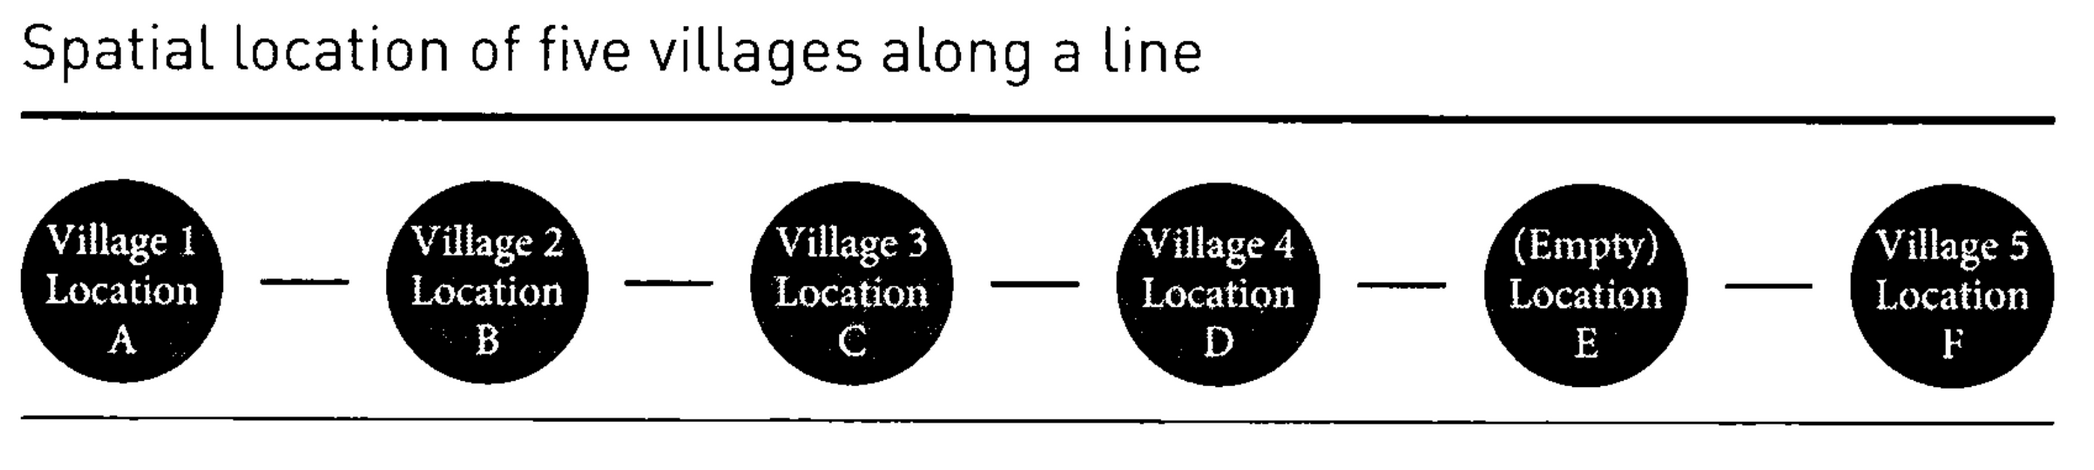
\includegraphics[width=0.9\textwidth,height=\textheight]{villages.png}

\begin{longtable}[]{@{}
  >{\raggedright\arraybackslash}p{(\columnwidth - 6\tabcolsep) * \real{0.2162}}
  >{\raggedright\arraybackslash}p{(\columnwidth - 6\tabcolsep) * \real{0.2162}}
  >{\raggedright\arraybackslash}p{(\columnwidth - 6\tabcolsep) * \real{0.3514}}
  >{\raggedright\arraybackslash}p{(\columnwidth - 6\tabcolsep) * \real{0.2162}}@{}}
\caption{Potential outcomes}\tabularnewline
\toprule\noalign{}
\begin{minipage}[b]{\linewidth}\raggedright
Village
\end{minipage} & \begin{minipage}[b]{\linewidth}\raggedright
Untreated (\(Y_{00}\))
\end{minipage} & \begin{minipage}[b]{\linewidth}\raggedright
Adjacent village treated (\(Y_{10}\))
\end{minipage} & \begin{minipage}[b]{\linewidth}\raggedright
Treated (\(Y_{01}\))
\end{minipage} \\
\midrule\noalign{}
\endfirsthead
\toprule\noalign{}
\begin{minipage}[b]{\linewidth}\raggedright
Village
\end{minipage} & \begin{minipage}[b]{\linewidth}\raggedright
Untreated (\(Y_{00}\))
\end{minipage} & \begin{minipage}[b]{\linewidth}\raggedright
Adjacent village treated (\(Y_{10}\))
\end{minipage} & \begin{minipage}[b]{\linewidth}\raggedright
Treated (\(Y_{01}\))
\end{minipage} \\
\midrule\noalign{}
\endhead
\bottomrule\noalign{}
\endlastfoot
A & 0 & 2 & 0 \\
B & 6 & 2 & 10 \\
C & 0 & 4 & 4 \\
D & 6 & 6 & 6 \\
F & 6 & NA & 3 \\
\end{longtable}

\begin{longtable}[]{@{}
  >{\raggedright\arraybackslash}p{(\columnwidth - 16\tabcolsep) * \real{0.1111}}
  >{\raggedright\arraybackslash}p{(\columnwidth - 16\tabcolsep) * \real{0.1111}}
  >{\raggedright\arraybackslash}p{(\columnwidth - 16\tabcolsep) * \real{0.1111}}
  >{\raggedright\arraybackslash}p{(\columnwidth - 16\tabcolsep) * \real{0.1111}}
  >{\raggedright\arraybackslash}p{(\columnwidth - 16\tabcolsep) * \real{0.1111}}
  >{\raggedright\arraybackslash}p{(\columnwidth - 16\tabcolsep) * \real{0.1111}}
  >{\raggedright\arraybackslash}p{(\columnwidth - 16\tabcolsep) * \real{0.1111}}
  >{\raggedright\arraybackslash}p{(\columnwidth - 16\tabcolsep) * \real{0.1111}}
  >{\raggedright\arraybackslash}p{(\columnwidth - 16\tabcolsep) * \real{0.1111}}@{}}
\caption{Probability of receiving treatment, spillover, and
control}\tabularnewline
\toprule\noalign{}
\begin{minipage}[b]{\linewidth}\raggedright
Village
\end{minipage} & \begin{minipage}[b]{\linewidth}\raggedright
A
\end{minipage} & \begin{minipage}[b]{\linewidth}\raggedright
B
\end{minipage} & \begin{minipage}[b]{\linewidth}\raggedright
C
\end{minipage} & \begin{minipage}[b]{\linewidth}\raggedright
D
\end{minipage} & \begin{minipage}[b]{\linewidth}\raggedright
F
\end{minipage} & \begin{minipage}[b]{\linewidth}\raggedright
Pr(control)
\end{minipage} & \begin{minipage}[b]{\linewidth}\raggedright
Pr(spillover)
\end{minipage} & \begin{minipage}[b]{\linewidth}\raggedright
Pr(treatment)
\end{minipage} \\
\midrule\noalign{}
\endfirsthead
\toprule\noalign{}
\begin{minipage}[b]{\linewidth}\raggedright
Village
\end{minipage} & \begin{minipage}[b]{\linewidth}\raggedright
A
\end{minipage} & \begin{minipage}[b]{\linewidth}\raggedright
B
\end{minipage} & \begin{minipage}[b]{\linewidth}\raggedright
C
\end{minipage} & \begin{minipage}[b]{\linewidth}\raggedright
D
\end{minipage} & \begin{minipage}[b]{\linewidth}\raggedright
F
\end{minipage} & \begin{minipage}[b]{\linewidth}\raggedright
Pr(control)
\end{minipage} & \begin{minipage}[b]{\linewidth}\raggedright
Pr(spillover)
\end{minipage} & \begin{minipage}[b]{\linewidth}\raggedright
Pr(treatment)
\end{minipage} \\
\midrule\noalign{}
\endhead
\bottomrule\noalign{}
\endlastfoot
1 & \(Y_{01}\) & \(Y_{10}\) & \(Y_{00}\) & \(Y_{00}\) & \(Y_{00}\) & 0.6
& 0.2 & 0.2 \\
2 & \(Y_{10}\) & \(Y_{01}\) & \(Y_{10}\) & \(Y_{00}\) & \(Y_{00}\) & 0.4
& 0.4 & 0.2 \\
3 & \(Y_{00}\) & \(Y_{10}\) & \(Y_{01}\) & \(Y_{10}\) & \(Y_{00}\) & 0.4
& 0.4 & 0.2 \\
4 & \(Y_{00}\) & \(Y_{00}\) & \(Y_{00}\) & \(Y_{10}\) & \(Y_{01}\) & 0.6
& 0.2 & 0.2 \\
5 & \(Y_{00}\) & \(Y_{00}\) & \(Y_{00}\) & \(Y_{00}\) & \(Y_{01}\) & 0.8
& 0 & 0.2 \\
\end{longtable}

Using these data, calculate the following quantities:

\begin{enumerate}
\def\labelenumi{\arabic{enumi}.}
\tightlist
\item
  Estimate \(E[Y_{01} - Y_{00}]\) for the random assignment that places
  the treatment at location A.
\end{enumerate}

To estimate ( E{[}Y\_\{01\} - Y\_\{00\}{]} ) for the random assignment
that places the treatment at location A, we focus on the villages that
are actually treated in that specific assignment. According to the
assignment table, when the clinic is placed in village A (Assignment 1),
only village A receives the treatment. The rest of the villages are
either in control or receive a spillover effect.

We then look at the potential outcomes table to determine the difference
in outcomes for village A between being treated and being untreated. For
village A, the outcome under treatment (( Y\_\{01\} )) is 0, and the
outcome under control with no adjacent village treated (( Y\_\{00\} ))
is also 0. Therefore, the treatment effect for village A is:

{[} Y\_\{01\} - Y\_\{00\} = 0 - 0 = 0 {]}

Since village A is the only treated village in this assignment, the
average treatment effect across treated villages is simply 0.

\textbf{Thus, the estimate of ( E{[}Y\_\{01\} - Y\_\{00\}{]} ) for the
assignment where treatment is placed at village A is 0.}

\begin{enumerate}
\def\labelenumi{\arabic{enumi}.}
\setcounter{enumi}{1}
\tightlist
\item
  Estimate \(E[Y_{10} - Y_{00}]\) for the random assignment that places
  the treatment at location A, restricting the sample to the set of
  villages that have a non-zero probability of expressing both of these
  potential outcomes.
\end{enumerate}

To estimate ( E{[}Y\_\{10\} - Y\_\{00\}{]} ) for the random assignment
that places the treatment at village A, we are interested in
understanding the \textbf{spillover effect}---that is, the effect on a
village of having a neighboring village receive treatment, compared to
receiving no treatment and having no neighboring village treated.

We are instructed to \textbf{restrict the sample} to only those villages
that have a \textbf{non-zero probability} of experiencing both the
control condition (( Y\_\{00\} )) and the spillover condition ((
Y\_\{10\} )) at some point across the five possible random assignments.
This ensures we are only comparing villages for which both outcomes are
relevant and could theoretically be observed under the experimental
design.

From the table of assignments, we identify that villages \textbf{A, B,
C, and D} each have some probability of receiving both ( Y\_\{00\} ) and
( Y\_\{10\} ) across the assignments. Village F, on the other hand,
never receives ( Y\_\{10\} ), so it is excluded from this estimation.

We then refer to the potential outcomes table to compute the difference
( Y\_\{10\} - Y\_\{00\} ) for each eligible village:

\begin{itemize}
\tightlist
\item
  Village A: ( 2 - 0 = 2 )
\item
  Village B: ( 2 - 6 = -4 )
\item
  Village C: ( 4 - 0 = 4 )
\item
  Village D: ( 6 - 6 = 0 )
\end{itemize}

Next, we calculate the average of these differences:

{[} \frac{2 + (-4) + 4 + 0}{4} = \frac{2}{4} = 0.5 {]}

Therefore, the estimated value of ( E{[}Y\_\{10\} - Y\_\{00\}{]} ) for
the assignment that places the treatment at village A, restricted to
villages that can experience both outcomes, is \textbf{0.5}.

\begin{enumerate}
\def\labelenumi{\arabic{enumi}.}
\setcounter{enumi}{2}
\tightlist
\item
  In order to make a more direct comparison between these two treatment
  effects, estimate \(E[Y_{01} - Y_{00}]\), restricting the sample to
  the same set of villages as in question 3.
\end{enumerate}

To estimate ( E{[}Y\_\{01\} - Y\_\{00\}{]} ), we are interested in the
\textbf{expected change in the outcome ( Y )} when a unit (in this case,
a village) moves from no treatment in either period (denoted by (
Y\_\{00\} )) to receiving the treatment only in the second period
(denoted by ( Y\_\{01\} )). In other words, we want to measure the
effect of introducing the treatment in the second period, for villages
that were untreated in the first.

To make this a \textbf{direct and fair comparison}, we restrict the
sample to the \textbf{same set of villages used in the prior comparison}
in Question 3. This typically means focusing on a \textbf{balanced
panel} of villages that are observed in both periods and belong to the
appropriate treatment group(s). Specifically, this subset should consist
of villages that:

\begin{enumerate}
\def\labelenumi{\arabic{enumi}.}
\tightlist
\item
  Were untreated in the first period, and
\item
  Either remained untreated in the second period or began receiving the
  treatment in the second period.
\end{enumerate}

By narrowing the sample in this way, we \textbf{control for
village-specific characteristics} that could confound the treatment
effect. The estimation of ( E{[}Y\_\{01\} - Y\_\{00\}{]} ) can then
proceed as a \textbf{difference in means} between the outcomes of these
two groups in the second period, assuming parallel trends.

This estimate gives us a \textbf{cleaner, more interpretable} measure of
the \textbf{impact of initiating the treatment}, isolated from other
dynamics that may affect villages not included in the restricted sample.

\begin{enumerate}
\def\labelenumi{\arabic{enumi}.}
\setcounter{enumi}{3}
\tightlist
\item
  Compare and contrast the advantages and disadvantages of using buffer
  rows versus clustered randomization in field experiments. Using the
  villages experiment as an example, discuss how each approach would
  affect: (1) the ability to estimate direct treatment effects, (2) the
  ability to study spillover effects, and (3) the complexity of
  statistical analysis required. What factors should researchers
  consider when choosing between these approaches?
\end{enumerate}

Buffer rows and clustered randomization are both strategies used in
field experiments to manage treatment spillovers, but they differ
significantly in design and implications. Buffer rows involve leaving
units (like villages or households) near treated units intentionally
untreated, creating a spatial ``buffer'' to reduce contamination from
treatment spillovers. This approach improves the ability to estimate
\textbf{direct treatment effects} by minimizing interference between
treated and control units. However, it reduces the number of units that
can receive the treatment, potentially lowering statistical power.
Clustered randomization, on the other hand, assigns entire clusters
(e.g., villages or regions) to either treatment or control, which helps
to contain spillovers within clusters. While this allows for cleaner
estimation of direct effects \textbf{at the cluster level}, it assumes
that spillovers don't cross cluster boundaries---an assumption that may
not always hold in practice.

In terms of studying \textbf{spillover effects}, buffer rows are often
less helpful because they are designed to \emph{prevent} spillovers
rather than measure them. Clustered designs, however, can be leveraged
to study spillovers if researchers collect data on untreated units
within treated clusters. This design enables the estimation of
\textbf{indirect effects} or externalities of the intervention.
Regarding \textbf{statistical complexity}, buffer rows can allow for
simpler analyses since the assumption of no interference is more likely
to hold. In contrast, clustered randomization requires more advanced
statistical methods---such as accounting for intra-cluster correlation
and using hierarchical models---which can complicate analysis and reduce
precision. Researchers must weigh these trade-offs based on the nature
of the intervention, the likelihood and importance of spillovers,
logistical constraints, and the main outcomes of interest when deciding
which approach is most appropriate.

\begin{enumerate}
\def\labelenumi{\arabic{enumi}.}
\setcounter{enumi}{4}
\tightlist
\item
  In class, we also examined a waitlist experiment that analyses the
  impact of TV campaigns on politicians' approval ratings. It is
  described in the slides and on pages 276 to 281. The tables related to
  the experiment are shown below and on page 279. Estimate
  \(E[Y_{01} - Y_{00}]\) by restricting your attention to weeks 2 and 3.
  How does this estimate compare to the estimate of
  \(E[Y_{11} - Y_{00}]\) presented in the text, which is also identified
  using observations from weeks 2 and 3?
\end{enumerate}

\begin{longtable}[]{@{}llll@{}}
\caption{Assigned treatment condition}\tabularnewline
\toprule\noalign{}
Market & Week 1 & Week 2 & Week 3 \\
\midrule\noalign{}
\endfirsthead
\toprule\noalign{}
Market & Week 1 & Week 2 & Week 3 \\
\midrule\noalign{}
\endhead
\bottomrule\noalign{}
\endlastfoot
1 & 01 & 11 & 11 \\
2 & 00 & 00 & 01 \\
3 & 00 & 01 & 11 \\
4 & 00 & 00 & 01 \\
5 & 00 & 00 & 00 \\
6 & 01 & 11 & 11 \\
7 & 00 & 00 & 00 \\
8 & 00 & 01 & 11 \\
\end{longtable}

\begin{longtable}[]{@{}llll@{}}
\caption{Observed outcomes}\tabularnewline
\toprule\noalign{}
Market & Week 1 & Week 2 & Week 3 \\
\midrule\noalign{}
\endfirsthead
\toprule\noalign{}
Market & Week 1 & Week 2 & Week 3 \\
\midrule\noalign{}
\endhead
\bottomrule\noalign{}
\endlastfoot
1 & 7 & 9 & 4 \\
2 & 7 & 5 & 7 \\
3 & 1 & 2 & 10 \\
4 & 4 & 3 & 10 \\
5 & 3 & 3 & 3 \\
6 & 10 & 8 & 10 \\
7 & 2 & 3 & 4 \\
8 & 3 & 1 & 3 \\
\end{longtable}

\begin{longtable}[]{@{}llll@{}}
\caption{Probabilities of assignment to treatment condition, by
week}\tabularnewline
\toprule\noalign{}
Treatment Condition & Week 1 & Week 2 & Week 3 \\
\midrule\noalign{}
\endfirsthead
\toprule\noalign{}
Treatment Condition & Week 1 & Week 2 & Week 3 \\
\midrule\noalign{}
\endhead
\bottomrule\noalign{}
\endlastfoot
Pr(00) & 0.75 & 0.50 & 0.25 \\
Pr(01) & 0.25 & 0.25 & 0.25 \\
Pr(11) & 0 & 0.25 & 0.50 \\
\end{longtable}

To estimate ( E{[}Y\_\{01\} - Y\_\{00\}{]} ), we focus only on weeks 2
and 3 and restrict our attention to markets that were either in the 00
(no treatment) or 01 (just began treatment) condition during those
weeks. In week 2, markets 2, 4, 5, and 7 were assigned 00 with an
average approval rating of 3.5, while markets 3 and 8 were assigned 01
with an average of 1.5. In week 3, markets 5 and 7 remained in condition
00 (average: 3.5), while markets 2 and 4 entered 01 (average: 8.5).
Pooling across both weeks, the average outcome for the 00 condition is
3.5, and for the 01 condition it is 5.0. Thus, the estimated treatment
effect of initiating the campaign is ( E{[}Y\_\{01\} - Y\_\{00\}{]} =
5.0 - 3.5 = 1.5 ).

This estimate can be directly compared to the estimate of (
E{[}Y\_\{11\} - Y\_\{00\}{]} ), which represents the effect of sustained
exposure to the campaign and is given as 3.0 in the text. The smaller
effect of ( E{[}Y\_\{01\} - Y\_\{00\}{]} ) suggests that the campaign's
impact grows over time---initial exposure provides some benefit, but the
full effect appears to require continued treatment. This distinction
highlights the importance of both timing and duration in assessing the
effectiveness of interventions like media campaigns.

\begin{enumerate}
\def\labelenumi{\arabic{enumi}.}
\setcounter{enumi}{6}
\tightlist
\item
  Experiments studying spillovers can raise unique ethical
  considerations. Discuss some of the ethical dilemmas that might arise
  when conducting experiments in the presence of interference. How can
  researchers design and implement spillover experiments in an ethically
  responsible manner?
\end{enumerate}

Experiments that study spillovers---where the treatment given to one
group affects others---can raise several ethical concerns. A primary
dilemma is the \textbf{unintended exposure} of untreated individuals to
the treatment's effects, which may violate principles of informed
consent. For example, in public health interventions or media campaigns,
individuals in the control group might still be indirectly affected,
blurring the lines of what they agreed to. Another concern arises when
\textbf{spillovers create unequal benefits or harms}: individuals in the
treatment group may benefit more, while those in the control or
spillover-affected groups receive less or even negative externalities,
raising issues of justice and fairness. These dynamics challenge the
ethical standard of equipoise---the idea that researchers do not know in
advance who will benefit more.

To ethically design experiments with potential spillovers, researchers
must first \textbf{acknowledge and anticipate interference} when seeking
consent and evaluating risks. One responsible approach is
\textbf{transparent communication}: informing participants that the
intervention could affect others beyond the treated group. Another is to
use \textbf{clustered randomization} or include \textbf{buffer zones} to
manage spillovers more deliberately and reduce unintended exposure.
Researchers should also perform \textbf{ethical impact assessments} that
consider the broader community---not just direct participants---and
incorporate these considerations into the study's design and reporting.
Finally, wherever possible, they should aim to \textbf{measure and
report spillover effects}, so that benefits and harms can be fairly
evaluated and shared, especially if the findings inform policy.

\begin{enumerate}
\def\labelenumi{\arabic{enumi}.}
\setcounter{enumi}{7}
\tightlist
\item
  How does the presence of interference affect the statistical power of
  a field experiment? In what ways might researchers need to adjust
  their sample size calculations when designing experiments where
  interference is anticipated?
\end{enumerate}

The presence of interference---where one unit's treatment affects
another unit's outcome---can significantly reduce the
\textbf{statistical power} of a field experiment. This is because
interference violates the assumption of \textbf{independent potential
outcomes}, which underpins standard hypothesis tests and variance
estimations. When untreated units are indirectly exposed to treatment
through spillovers, the difference between treatment and control groups
becomes \textbf{less distinct}, making it harder to detect true effects.
In other words, interference can dilute the average treatment effect,
inflate variance, and increase the chance of Type II errors (failing to
detect a real effect).

To address these challenges, researchers need to \textbf{adjust their
sample size calculations} by accounting for the structure and degree of
interference. One common strategy is to \textbf{design experiments at
the cluster level}, grouping units in such a way that interference
happens mostly within clusters rather than between them. In this case,
the \textbf{intracluster correlation (ICC)} must be factored into power
calculations, which usually results in the need for a \textbf{larger
sample size} to maintain sufficient power. Researchers may also simulate
potential interference scenarios or use \textbf{network-based models} to
estimate how spillovers could influence outcomes and sample size needs.
Planning for interference in advance allows for more realistic
expectations about statistical precision and helps ensure that the study
remains adequately powered.

\begin{enumerate}
\def\labelenumi{\arabic{enumi}.}
\setcounter{enumi}{8}
\tightlist
\item
  Sometimes researchers are reluctant to randomly assign individual
  students in elementary classrooms because they are concerned that
  treatments administered to some students are likely to spill over to
  untreated students in the same classroom. In an attempt to get around
  possible violations of the non-interference assumption, they assign
  classrooms as clusters to treatment and control, and administer the
  treatment to all students in a classroom.
\end{enumerate}

\begin{enumerate}
\def\labelenumi{(\alph{enumi})}
\item
  State the non-interference assumption as it applies to the proposed
  clustered design.
\item
  What causal estimand does the clustered design identify? Does this
  causal estimand include or exclude spillovers within classrooms?
\end{enumerate}

\textbf{(a)} In the context of the proposed clustered design, the
\textbf{non-interference assumption}---also known as the \textbf{Stable
Unit Treatment Value Assumption (SUTVA)}---requires that the outcome for
any student depends \textbf{only on the treatment status of their own
classroom}, and \textbf{not on the treatment status of students in other
classrooms}. That is, there is \textbf{no interference across clusters}:
a student's outcome is assumed to be unaffected by whether students in
other classrooms receive the treatment. However, this design explicitly
allows for, or even expects, potential spillovers \textbf{within}
classrooms by treating entire classrooms uniformly.

\textbf{(b)} This clustered design identifies the \textbf{average
treatment effect of assigning a classroom to the treatment condition},
often called the \textbf{intention-to-treat (ITT) effect at the cluster
level}. Importantly, this causal estimand \textbf{includes}
within-classroom spillovers: it captures the combined effect of
\textbf{direct exposure to the treatment and any peer effects}
experienced within the classroom. It does not separate these components.
By contrast, it \textbf{excludes} spillovers between classrooms,
assuming none exist. This design is well-suited for capturing the
\textbf{overall effect of implementing a treatment at the classroom
level}, but it does not identify the isolated effect of individual
treatment exposure absent peer influence.

\begin{enumerate}
\def\labelenumi{\arabic{enumi}.}
\setcounter{enumi}{9}
\tightlist
\item
  If an experiment is conducted in a setting with significant
  interference, how does this affect the generalisability of the
  findings to other settings where the nature or extent of interference
  might be different? Discuss the challenges and potential strategies
  for increasing the external validity of experimental findings when
  interference is a concern.
\end{enumerate}

When interference is significant in an experimental setting, it
complicates the \textbf{generalizability (external validity)} of the
findings because the treatment effect is context-dependent. The measured
outcomes in such settings reflect not only the direct effect of the
treatment but also the pattern and intensity of spillovers among
units---factors that may vary widely in other environments. For
instance, an intervention that relies heavily on peer influence may
appear more effective in tightly knit communities or classrooms but
yield weaker results in more dispersed or disconnected groups. If the
structure of social networks or proximity among units differs across
settings, the estimated effect from the original study may \textbf{not
translate well elsewhere}.

To address these challenges and improve external validity, researchers
can adopt several strategies. One is to \textbf{explicitly model and
measure the network or spatial structure} through which interference
occurs, allowing for better interpretation and comparison across
contexts. Another strategy is to \textbf{conduct the experiment across
diverse settings} (e.g., different schools, neighborhoods, or regions)
to examine how treatment effects vary with the intensity of
interference. Researchers can also perform \textbf{sensitivity analyses
or simulations} to estimate how changes in spillover patterns might
affect outcomes. Finally, clearly \textbf{documenting the mechanisms of
interference} and the conditions under which the experiment was
conducted allows other researchers and policymakers to better judge how
relevant the findings are to their own contexts.




\end{document}
